\documentclass[12pt,a4paper]{article}

% ─── Page Layout ───────────────────────────────────────────────────────────────
\usepackage[a4paper, margin=0.8in, headheight=14pt]{geometry}

% ─── Fonts (XeLaTeX) ───────────────────────────────────────────────────────────
\usepackage{fontspec}
\usepackage{unicode-math}
\setmainfont{TeX Gyre Pagella}
\setmonofont[Scale=0.88]{TeX Gyre Cursor}
\setmathfont{Latin Modern Math}

% ─── Packages ──────────────────────────────────────────────────────────────────
\usepackage{xcolor}
\usepackage{colortbl}
\usepackage{titlesec}
\usepackage{enumitem}
\usepackage{tabularx}
\usepackage{booktabs}
\usepackage{array}
\usepackage{amsmath}
\usepackage{tikz}
\usetikzlibrary{shapes.geometric, arrows.meta, positioning, calc, fit, decorations.pathreplacing}
\usepackage{tcolorbox}
\tcbuselibrary{skins, breakable}
\usepackage{hyperref}
\usepackage{fancyhdr}
\usepackage{graphicx}
\usepackage{microtype}
\hyphenpenalty=10000
\exhyphenpenalty=10000
\sloppy
\usepackage{caption}
\usepackage{setspace}
\usepackage{multirow}
\usepackage{tocloft}

% ─── Q&A helper ────────────────────────────────────────────────────────────────
\newcommand{\Q}[1]{\textbf{#1}\par\noindent\ignorespaces}

% ─── Colour Palette ────────────────────────────────────────────────────────────
\definecolor{myred}{RGB}{196,30,58}
\definecolor{mydark}{RGB}{30,30,50}
\definecolor{mygreen}{RGB}{14,120,80}
\definecolor{myteal}{RGB}{0,130,140}
\definecolor{myamber}{RGB}{180,100,0}
\definecolor{mypurple}{RGB}{100,30,160}
\definecolor{mygray}{RGB}{246,247,249}
\definecolor{mgframe}{RGB}{180,185,200}
\definecolor{watermark}{RGB}{145,150,170}
\definecolor{hdrred}{RGB}{250,232,235}
\definecolor{hdrgreen}{RGB}{220,244,233}
\definecolor{hdrteal}{RGB}{220,242,244}
\definecolor{hdramber}{RGB}{253,242,215}
\definecolor{hdrpurple}{RGB}{238,228,255}
\definecolor{hdrgray}{RGB}{238,240,245}
\definecolor{rowalt}{RGB}{250,251,253}

% ─── Section Formatting ────────────────────────────────────────────────────────
\titleformat{\section}
  {\large\bfseries\color{myred}}{\thesection.}{0.5em}{}
  [\vspace{1pt}{\color{myred}\rule{\linewidth}{0.8pt}}]
\titleformat{\subsection}
  {\normalsize\bfseries\color{myteal}}{\thesubsection}{0.5em}{}
\titlespacing*{\section}{0pt}{18pt}{7pt}
\titlespacing*{\subsection}{0pt}{11pt}{4pt}

% ─── Paragraph ─────────────────────────────────────────────────────────────────
\setlength{\parindent}{0pt}
\setlength{\parskip}{4pt}

% ─── TOC Styling ───────────────────────────────────────────────────────────────
\renewcommand{\cfttoctitlefont}{\large\bfseries\color{myred}}
\renewcommand{\cftaftertoctitle}{\par\noindent{\color{myred}\rule{\linewidth}{0.8pt}}}
\setlength{\cftbeforetoctitleskip}{0pt}
\setlength{\cftaftertoctitleskip}{6pt}
\renewcommand{\cftsecfont}{\normalsize\bfseries\color{mydark}}
\renewcommand{\cftsecpagefont}{\normalsize\bfseries\color{mydark}}
\renewcommand{\cftsecleader}{\cftdotfill{\cftdotsep}}
\setlength{\cftbeforesecskip}{7pt}
\renewcommand{\cftsubsecfont}{\small\color{mydark}}
\renewcommand{\cftsubsecpagefont}{\small\color{mydark}}
\setlength{\cftbeforesubsecskip}{3pt}
\setlength{\cftsubsecindent}{1.4em}

% ─── Table helpers ─────────────────────────────────────────────────────────────
\renewcommand{\arraystretch}{1.45}
\setlength{\tabcolsep}{6pt}
\arrayrulecolor{mydark}
\newcolumntype{B}[1]{>{\small\bfseries\raggedright\arraybackslash}m{#1}}
\newcolumntype{Y}{>{\small\raggedright\arraybackslash}X}
\renewcommand{\tabularxcolumn}[1]{m{#1}}

% ─── Header / Footer ───────────────────────────────────────────────────────────
\pagestyle{fancy}
\fancyhf{}
\fancyhead[L]{\small\color{myred}\textbf{PE-EC701B}\;\color{mydark}--- Satellite Communication}
\fancyhead[R]{\small\color{myteal}\textbf{Module 1 Notes}}
\fancyfoot[C]{\small\color{mydark}\thepage}
\fancyfoot[R]{\small\color{watermark}\textit{\copyright\ Biraj}}
\renewcommand{\headrulewidth}{0.5pt}
\renewcommand{\footrulewidth}{0.3pt}

% ─── Hyperref ──────────────────────────────────────────────────────────────────
\hypersetup{
  colorlinks=true, linkcolor=myteal, urlcolor=myteal,
  pdfauthor={Biraj Sarkar},
  pdftitle={PE-EC701B --- Module 1 Notes}
}

% ─── tcolorbox styles ──────────────────────────────────────────────────────────
\tcbset{
  tikzbox/.style={
    colback=mygray, colframe=mgframe, boxrule=0.6pt, arc=4pt,
    left=8pt, right=8pt, top=6pt, bottom=6pt,
    colbacktitle=mgframe, coltitle=mydark,
    fonttitle=\small\bfseries
  },
  defbox/.style={
    colback=hdrgreen, colframe=mygreen, boxrule=0.8pt, arc=4pt,
    left=9pt, right=9pt, top=6pt, bottom=6pt,
    colbacktitle=mygreen, coltitle=white,
    fonttitle=\small\bfseries
  },
  formulabox/.style={
    colback=hdrteal, colframe=myteal, boxrule=0.8pt, arc=4pt,
    left=9pt, right=9pt, top=7pt, bottom=7pt,
    colbacktitle=myteal, coltitle=white,
    fonttitle=\small\bfseries
  },
  examplebox/.style={
    colback=hdramber, colframe=myamber, boxrule=0.8pt, arc=4pt,
    left=9pt, right=9pt, top=6pt, bottom=6pt,
    colbacktitle=myamber, coltitle=white,
    fonttitle=\small\bfseries
  },
  masonbox/.style={
    colback=hdrpurple, colframe=mypurple, boxrule=0.8pt, arc=4pt,
    left=9pt, right=9pt, top=6pt, bottom=6pt,
    colbacktitle=mypurple, coltitle=white,
    fonttitle=\small\bfseries
  },
  exambox/.style={
    colback=hdrpurple, colframe=mypurple, boxrule=1pt, arc=5pt,
    left=10pt, right=10pt, top=8pt, bottom=8pt,
    colbacktitle=mypurple, coltitle=white,
    fonttitle=\bfseries,
    breakable, title after break={\textbf{Frequently Asked / Viva Questions (contd.)}}}
}
% Make all boxes breakable across pages
\tcbset{breakable}

% ─── TikZ styles ───────────────────────────────────────────────────────────────
\tikzset{
  block/.style={rectangle, draw=myteal, fill=hdrteal,
    text width=2.4cm, align=center, minimum height=0.95cm,
    font=\small, rounded corners=3pt, line width=0.7pt},
  redblock/.style={rectangle, draw=myred, fill=hdrred,
    text width=2.4cm, align=center, minimum height=0.95cm,
    font=\small, rounded corners=3pt, line width=0.7pt},
  netnode/.style={rectangle, draw=myteal, fill=hdrteal,
    text width=1.5cm, align=center, minimum height=0.8cm,
    font=\small, rounded corners=3pt, line width=0.7pt},
  sumjunc/.style={circle, draw=myamber, fill=hdramber,
    minimum size=0.62cm, font=\small, line width=0.8pt},
  snode/.style={circle, draw=mypurple, fill=hdrpurple,
    minimum size=0.55cm, font=\footnotesize, line width=0.7pt},
  arrow/.style={-Stealth, thick, color=mydark},
  redarrow/.style={-Stealth, thick, color=myred},
  line/.style={thick, color=mydark}
}

% ═══════════════════════════════════════════════════════════════════════════════
\begin{document}
% ═══════════════════════════════════════════════════════════════════════════════

\begin{center}
  {\LARGE\bfseries\color{myred} PE-EC701B --- Satellite Communication}\\[5pt]
  {\normalsize\color{mydark} Semester VII \quad$\bullet$\quad 3L:0T:0P \quad$\bullet$\quad 3 Credits}\\[3pt]
  {\normalsize\color{myteal}\textbf{Module 1 Exam Notes: Introduction to Satellite Communication}}\\[3pt]
  {\small\color{mydark} CGEC \;$|$\; B.Tech ECE (2023--27) \;$|$\; \textit{Biraj Sarkar}}
\end{center}
\vspace{2pt}
\noindent{\color{myred}\rule{\linewidth}{1.5pt}}
\vspace{2pt}

\hypersetup{linkcolor=mydark}
\tableofcontents
\hypersetup{linkcolor=myteal}
\newpage

% ===============================================================================
\section{Principles of Satellite Communication}
% ===============================================================================

Satellite communication is the transmission of information between terrestrial stations using an artificial satellite positioned in Earth's orbit as an active relay. The satellite acts as an orbit-based radio repeater (transponder) that receives signals from one ground station, processes them, and retransmits them to other ground stations.

\begin{tcolorbox}[defbox]
\textbf{Satellite Communication:} A system where an orbiting spacecraft serves as an active wireless relay station. It receives line-of-sight uplink radio signals at frequency $f_u$ from an Earth station, amplifies and translates them to downlink frequency $f_d$, and broadcasts them back to Earth stations.
\end{tcolorbox}

\subsection{Basic Principles of Operation}
The operational principles of a satellite communications system are governed by the following sequence:
\begin{enumerate}[label=\textbf{\arabic*.}, leftmargin=*, itemsep=3pt]
  \item \textbf{Uplink Transmission:} Terrestrial transmitter sends a modulated high-frequency carrier wave (typically in GHz) toward the satellite using a high-gain directional dish antenna.
  \item \textbf{Frequency Translation:} The satellite transponder down-converts the incoming signal to a lower frequency. This translation is vital because it prevents the high-power downlink signal from feeding back and jamming the sensitive uplink receiver.
  \item \textbf{Downlink Transmission:} The converted signal is amplified (via traveling-wave tubes or solid-state power amplifiers) and beamed back to Earth using onboard directive antennas.
\end{enumerate}

\subsection{System Architecture}
The block diagram below details the basic architecture of a satellite communication system:

\begin{tcolorbox}[tikzbox, title={Satellite Communication System Architecture}]
\centering
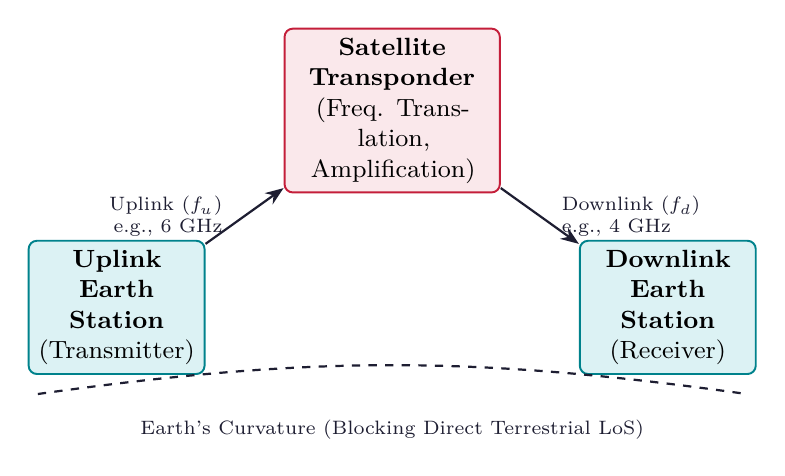
\begin{tikzpicture}[node distance=0.6cm and 1.2cm, every node/.style={font=\scriptsize}]
  % Ground Station Left
  \node[block, text width=2.0cm] (tx) at (0,0) {\textbf{Uplink Earth Station}\\(Transmitter)};
  
  % Satellite Node (Top Center)
  \node[redblock, text width=2.5cm] (sat) at (3.5,2.5) {\textbf{Satellite Transponder}\\(Freq. Translation,\\Amplification)};
  
  % Ground Station Right
  \node[block, text width=2.0cm] (rx) at (7.0,0) {\textbf{Downlink Earth Station}\\(Receiver)};
  
  % Arrows with frequency labels
  \draw[arrow] (tx) -- node[midway, left=0.15cm, align=right] {Uplink ($f_u$)\\e.g., 6 GHz} (sat);
  \draw[arrow] (sat) -- node[midway, right=0.15cm, align=left] {Downlink ($f_d$)\\e.g., 4 GHz} (rx);
  
  % Earth surface curve
  \draw[thick, color=mydark, dashed] (-1.0,-1.1) to[out=8, in=172] (8.0,-1.1);
  \node[below, align=center, color=mydark] at (3.5,-1.3) {Earth's Curvature (Blocking Direct Terrestrial LoS)};
\end{tikzpicture}
\end{tcolorbox}

% ===============================================================================
\section{Brief History of Satellite Systems}
% ===============================================================================

The theoretical concept of satellite communication was popularized by Arthur C. Clarke in 1945, who proposed using three geostationary satellites separated by $120^\circ$ to cover the entire globe. The operational milestones of satellite communication are outlined below:

\begin{itemize}[leftmargin=*, itemsep=3pt]
  \item \textbf{Sputnik 1 (1957):} Launched by the Soviet Union. It was the first artificial satellite in orbit, transmitting radio telemetry beeps at 20 MHz and 40 MHz.
  \item \textbf{Project Score (1958):} The first voice transmission satellite, launched by the United States. It broadcasted a pre-recorded Christmas message.
  \item \textbf{Echo 1 (1960):} A passive reflector balloon satellite that simply bounced radio signals off its metallized surface.
  \item \textbf{Telstar 1 (1962):} The first active, direct-amplifying communication satellite. It successfully transmitted live transatlantic television signals.
  \item \textbf{Syncom 3 (1964):} The first geostationary (GEO) communication satellite, which was used to broadcast the 1964 Tokyo Olympics.
  \item \textbf{Intelsat I (Early Bird, 1965):} The first commercial communications satellite, establishing regular telephone and TV traffic.
\end{itemize}

% ===============================================================================
\section{Advantages and Disadvantages of Satellite Communication}
% ===============================================================================

\textbf{Advantages:}
\begin{itemize}[leftmargin=*, itemsep=3pt]
  \item \textbf{Geographical Coverage:} A single geostationary satellite can cover up to 42.4\% of the Earth's surface. Only three satellites can cover the entire Earth (excluding polar regions).
  \item \textbf{Point-to-Multipoint Capability:} Ideal for broadcasting signals (e.g., satellite television) simultaneously to millions of receiving Earth terminals.
  \item \textbf{Independent of Terrestrial Infrastructure:} Highly reliable for emergency communications in rugged terrains, oceans, or disaster-struck areas where ground cables are non-existent or destroyed.
  \item \textbf{High Bandwidth:} Operates at high frequencies, providing large data capacity for television channels and broadband.
\end{itemize}

\textbf{Disadvantages:}
\begin{itemize}[leftmargin=*, itemsep=3pt]
  \item \textbf{Propagation Delay (Latency):} In Geostationary Earth Orbit (GEO), the round-trip distance is approximately 72,000 km, leading to a signal propagation latency of about 240 ms to 280 ms.
  \item \textbf{High Launch and Development Cost:} Designing, launching, and maintaining satellites in orbit requires massive capital investment and carries risks of launch failure.
  \item \textbf{No Servicing or Maintenance:} Once launched, satellites are generally impossible to service physically. Any hardware failure can render the entire system useless.
  \item \textbf{Vulnerability to Interference:} Subject to solar eclipse outages, atmospheric absorption, and radio frequency interference (RFI) from other terrestrial transmitters.
\end{itemize}

% ===============================================================================
\section{Applications of Satellite Communication}
% ===============================================================================

Satellite systems have permeated both civilian and military domains due to their global reach:

\begin{enumerate}[label=\textbf{\arabic*.}, leftmargin=*, itemsep=4pt]
  \item \textbf{Broadcast Television and Radio:} Direct-to-Home (DTH) satellite TV transmits digital programming directly to household dish antennas.
  \item \textbf{Satellite Telephony and Internet:} Inmarsat, Iridium, and Starlink systems provide satellite broadband and voice calls in remote, maritime, and aeronautical zones.
  \item \textbf{Global Navigation Satellite Systems (GNSS):} Systems like GPS (US), GLONASS (Russia), Galileo (EU), and NavIC (India) use orbital constellations to provide precise 3D positioning and timing.
  \item \textbf{Meteorology and Earth Observation:} Satellites track weather systems, hurricane paths, ocean temperatures, and environmental changes.
  \item \textbf{Military Reconnaissance and Tactical Comms:} Encrypted tactical communication links, troop tracking, drone navigation, and ballistic missile early warning networks.
\end{enumerate}

% ===============================================================================
\section{Frequency Bands Used for Satellite Communication}
% ===============================================================================

The International Telecommunication Union (ITU) regulates the allocation of frequencies to prevent mutual interference. Satellite links operate in microwave frequencies, allowing them to penetrate the Earth's ionosphere.

\subsection{Standard Frequency Band Classification}
The table below details the frequency bands used for satellite links:

\par\noindent
{\renewcommand{\arraystretch}{1.55}%
\begin{tabularx}{\linewidth}{|B{2.2cm}|>{\centering\arraybackslash}m{2.5cm}|>{\centering\arraybackslash}m{2.5cm}|Y|}
\hline
\textbf{Band} & \textbf{Uplink Range} & \textbf{Downlink Range} & \textbf{Key Advantages / Applications} \\[4pt]
\hline
\textbf{L Band} & $1.61 - 1.66$ GHz & $1.52 - 1.56$ GHz & Low attenuation, small antennas; GPS, mobile satellite terminals (Iridium). \\[4pt]
\hline
\textbf{S Band} & $2.1 - 2.3$ GHz & $1.9 - 2.1$ GHz & Minimal rain fade; Mobile satellite service, DTH audio broadcasting. \\[4pt]
\hline
\textbf{C Band} & $5.92 - 6.42$ GHz & $3.7 - 4.2$ GHz & Highly mature technology, low rain fade; Telephony, TV networks, VSAT systems. \\[4pt]
\hline
\textbf{X Band} & $7.9 - 8.4$ GHz & $7.25 - 7.75$ GHz & Highly secure, military exclusive; Reconnaissance, military communications. \\[4pt]
\hline
\textbf{Ku Band} & $14.0 - 14.5$ GHz & $11.7 - 12.2$ GHz & High gain, smaller dish size; DTH TV, VSAT networks, high-speed data. \\[4pt]
\hline
\textbf{Ka Band} & $27.5 - 31.0$ GHz & $17.7 - 21.2$ GHz & Massive bandwidth; Satellite broadband (Starlink, Viasat), high-throughput systems. \\[4pt]
\hline
\end{tabularx}
}

\subsection{Uplink vs. Downlink Frequency Separation}
In satellite systems, the uplink frequency ($f_u$) is \textbf{always higher} than the downlink frequency ($f_d$).
\begin{equation}
  f_u > f_d
\end{equation}
This design choice is guided by three main engineering reasons:
\begin{enumerate}[label=\textbf{\alph*.}, leftmargin=*, itemsep=2pt]
  \item \textbf{Atmospheric Loss Compensation:} Propagation attenuation (such as rain fade) increases with frequency. An Earth station has access to high-power grid electricity, allowing it to easily output high power to overcome these losses at higher uplink frequencies. The satellite, however, has a limited power budget (relying on solar panels and batteries) and must use the lower, less attenuated frequency ($f_d$) for its downlink broadcast to conserve power.
  \item \textbf{Antenna Gain and Size:} High frequencies yield smaller wavelengths ($\lambda$), allowing the Earth station to achieve a narrower, more focused uplink beam with a reasonably sized dish.
  \item \textbf{Feedback Prevention:} The frequency translation prevents electromagnetic feedback loop oscillations inside the satellite transponder.
\end{enumerate}

% ===============================================================================
% MANDATORY QUICK REVISION PAGE
% ===============================================================================
\newpage
\begin{center}
  {\large\bfseries\color{myred} Quick Revision --- Module I}\\[3pt]
  {\small\color{mydark} Introduction to Satellite Communication $|$ PE-EC701B}
\end{center}
\noindent{\color{myred}\rule{\linewidth}{1.2pt}}
\vspace{4pt}

\begin{tcolorbox}[formulabox, title={\textbf{Key Formulas at a Glance}}]
\renewcommand{\arraystretch}{1.3}
\begin{tabularx}{\linewidth}{B{4.5cm} X}
Wavelength-Frequency & $\lambda = \frac{c}{f}$ \quad ($c \approx 3 \times 10^8$ m/s) \\[6pt]
One-Way Latency & $t = \frac{d}{c}$ \quad ($d \approx 35,786$ km for GEO) \\[6pt]
Round-Trip Delay & $T_d = 2 \times \frac{d}{c} \approx 238 \text{ ms}$ (minimum orbital path) \\[6pt]
Uplink vs Downlink & $f_{\text{uplink}} > f_{\text{downlink}}$ \quad (e.g., $6/4$ GHz for C-band, $14/12$ GHz for Ku-band)
\end{tabularx}
\end{tcolorbox}

\begin{tcolorbox}[defbox, title={\textbf{One-Line Definitions}}]
\begin{itemize}[leftmargin=*, itemsep=2.5pt, topsep=0pt]
  \item \textbf{Satellite communication:} Orbiting radio transponders routing signals between distant Earth stations.
  \item \textbf{Transponder:} Spacecraft equipment that receives, converts, and transmits RF carriers.
  \item \textbf{Uplink:} The radio link transmitting from Earth stations to the satellite.
  \item \textbf{Downlink:} The radio link transmitting from the satellite to Earth stations.
  \item \textbf{Frequency Translation:} Conversion of uplink frequency to downlink frequency to avoid feedback.
  \item \textbf{Rain Fade:} Attenuation of microwave signals due to scattering and absorption by rain droplets.
  \item \textbf{GEO:} Geostationary Earth Orbit, located at an altitude of approximately 35,786 km.
\end{itemize}
\end{tcolorbox}

\begin{tcolorbox}[exambox, title={\textbf{Frequently Asked / Viva Questions}}]
\begin{enumerate}[topsep=0pt, label=\textbf{Q\arabic*.}, itemsep=5pt]
  \item \Q{State the fundamental principle of satellite communication.}
    It operates as a line-of-sight microwave link using an active orbiting transponder to receive, translate, and retransmit signals across massive global distances.
  \item \Q{Why is the uplink frequency always higher than the downlink frequency ($f_u > f_d$)?}
    Earth stations have abundant power to transmit at higher frequencies which suffer more atmospheric loss, whereas satellites have constrained onboard power and must transmit down at lower, less attenuated frequencies.
  \item \Q{Who first conceptualized global satellite communication using geostationary orbits?}
    Arthur C. Clarke, in a 1945 paper titled "Extra-Terrestrial Relays", proposing three GEO satellites.
  \item \Q{What is the function of a transponder on a satellite?}
    To receive the uplink signal, filter out noise, down-convert the frequency to the downlink band, and amplify it for retransmission.
  \item \Q{List standard frequency band designations and their typical frequencies.}
    C-band ($6/4$ GHz), Ku-band ($14/12$ GHz), Ka-band ($30/20$ GHz), and S-band ($2$ GHz).
  \item \Q{What are the main advantages of satellite communication over terrestrial networks?}
    Vast geographical coverage (up to 42.4\% per GEO satellite), point-to-multipoint broadcasting, and independent operational viability in remote/disaster areas.
  \item \Q{Explain the propagation delay disadvantage of GEO satellites.}
    Due to the high altitude (35,786 km), signals travel at the speed of light, yielding a round-trip Earth-satellite-Earth latency of approximately 240 ms to 280 ms.
  \item \Q{What was Sputnik 1?}
    The first artificial satellite, launched by the USSR in October 1957, transmitting simple telemetry beeps.
  \item \Q{What is rain fade, and in which frequency bands is it most prominent?}
    It is signal attenuation caused by rain droplets. It is highly prominent at frequencies above 10 GHz (Ku and Ka bands).
  \item \Q{What is GPS, and what are its orbital parameters?}
    Global Positioning System, a medium Earth orbit (MEO) constellation orbiting at an altitude of ~20,200 km, providing precise navigation.
  \item \Q{How many satellites are required for global coverage, and why?}
    Three geostationary satellites separated by $120^\circ$ of longitude because each satellite covers approximately 42.4\% of the Earth's surface.
  \item \Q{What is the difference between active and passive satellites?}
    Passive satellites (like Echo 1) only reflect signals. Active satellites (like Telstar 1) amplify and process signals.
\end{enumerate}
\tcbset{colbacktitle=myteal, coltitle=white}
\end{tcolorbox}

\begin{tcolorbox}[tikzbox, title={Comparison of Satellite Frequency Bands}]
\renewcommand{\arraystretch}{1.4}
\par\noindent
{\renewcommand{\arraystretch}{1.55}%
\begin{tabularx}{\linewidth}{|B{2.5cm}|Y|Y|Y|}
\hline
\textbf{Parameter} & \textbf{\color{myteal}C Band} & \textbf{\color{myred}Ku Band} & \textbf{\color{myamber}Ka Band} \\[4pt]
\hline
\textbf{Frequency (U/D)} & $6 / 4$ GHz & $14 / 12$ GHz & $30 / 20$ GHz \\
\hline
\textbf{Rain Fade} & Negligible / Low & Moderate & Very High \\
\hline
\textbf{Dish Antenna Size} & Large ($2.4 - 3.7$ m) & Small ($0.6 - 1.2$ m) & Very Small ($0.3 - 0.75$ m) \\[4pt]
\hline
\textbf{Applications} & Backhaul telephony, TV distribution, maritime links. & DTH satellite TV, home VSAT terminals. & Satellite broadband, high-throughput commercial services. \\[4pt]
\hline
\end{tabularx}
}
\end{tcolorbox}

\end{document}
